We propose an SLA guided, continuous data provision and integration approach that proposes three steps  starting from the processing of the request  to the delivery of the result sets.

Given a requirement expressing a query and quality of service preferences: cost, provenance, reputation, time the system processes it  as follows: (i) derived SLA  computation for filtering possible data providers; (ii) query rewriting for computing services compositions that can be used for building results; (iii) optimizing and integrating results. The output of these steps generate intermediate results that are stored as knowledge in order to reduce the overhead of the query evaluation process. The whole process is monitored to determine whether a computed SLA is being honoured while a query is evaluated. 
The following sections describe how this query is evaluated according to our approach. 





%-----------------------------------------------------------------
\subsection{Deriving a query SLA}
\label{sec:slaModel}
%-----------------------------------------------------------------

%\begin{itemize}
%\item Expression haut niveau du SLA en termes de préférences qui doit converger avec le SLA technique des services.
%  \begin{itemize}
%  \item (Souhait de temps de réponse, coût des services, espace de stockage,  
%  \item Templates pour exprimer le SLA
%  \item Intégration: modèle pivot de SLA
%\end{itemize}
%
%\item SLA violation contrôlée avec des mechanisms de monitoring.
%\item Que ce que devient l’intégration de données par rapport au SLA
%\item Création dynamique de SLA → niche de marché: étant donnée deux SLA fabriquer un SLA d’intégration
%\end{itemize}

The key and original aspect of   our proposed data integration and provision process is  defined as a vertical mapping of user QoS preferences and agreed SLAs. This  leads to a {\em derived SLA} that guides the evaluation of a query. A query has associated preferences  expressed as macroscopic constraints (i.e. user preferences statement): execution time, pay / no pay, data reliability, provenance, freshness, privacy, partial/full results, delivery mode. These constraints are coupled with the profile of the user which is in general stated in her cloud subscription (amount of assigned storage space, number of requests, I/O transfered Mega bytes, etc.). Given a query and its preferences statement, the system  finds  service compositions that produce results   meeting the required constraints. 

%One may think to a first filter to remove the individual services which do not meet some or all of the constraints expressed by the user. 

We assume that services export SLAs (i.e., agreed SLAs) that define measures  of finer granularity than those defined by the user.  The service SLA measures  are: response time, availability, price/call, reliability, data production rate. Other measures are associated to the conditions in which the service is called or to the precision and recall of their produced data given a request. These measures are, in general, computed by monitoring the execution and conversations associted to services. For example the cost of retrieving the list of energy providers within a region with their KWatt cost provided that calls cost between 0,25 - 0,50 euros depending on the data service. This request  includes the price of calling a service, plus the price of data transmision according to the amount of trasnmitted MegaOctets through the network and the type of subscription of the user for using the network. Since we assume that services can be deployed on different cloud providers, measures and SLA threasholds can vary.
 Measures can be also hybrid, in the sense that they can be statically stated partially but they require to be precised at execution time.  A service  agreed SLA is expressed through an  XML document using the specification WSLA (Web service level agreement \footnote{\footnotesize http://www.research.ibm.com/people/a/akeller/\-Data/WSLASpecV1-20030128.pdf}).


Given agreed SLA's and a user preferences statement the challenge is to compute a  {\em derived SLA} that  maps SLA measures and preferences attributes.  The derived SLA is defined as a set of measures that correspond to the user preferences computed as a function of different static, computed and hybrid measures. The {\em derived SLA}  will guide the way the query will be evaluated, and the way results will be computed and delivered.

 We propose a classification of SLA measures that represents the relationship between fine grained measures used by agreed SLAs and coarse grained measures used in user preferences statements. It specifies also how to compute coarse grained measures with fine grained ones. For example, data precision will be computed as a function of availability, freshness and provenance exported by data services. The derived SLA  can be seen as a set of inequations that have to be solved during the execution of a service composition. Since some of them can only be determined at execution time, the decision on which services will participate in the evaluation of the query is approximated. We will discuss this issue in the next sections.


This step may lead either to the rejection of integration in case of total incompatibility, or to a negotiation between SLA which will lead us to the proposal for a negotiated SLA integration and thus the need for an adaptive setting.
%
%
% \begin{enumerate}
%\item Computation of a global SLA given the existing possible SLA agreed by data providers that can be called for answering the query. Data providers are filtered in this way, since only those agreed SLA that can be combined into a global SLA that can fulfill the user preferences are considered for retrieving data.
%
 % 
%  \item Filter the data providers that can potentially participate in the evaluation of the query taking into consideration the preferences associated to the query.
  %
 % \item 
 Negociation of this type of SLA depends strongly on the request sent and the services deployed at the arrival time of the application on the cloud. This negotiation can be expensive and may not scale well.
 % \end{enumerate}


%-----------------------------------------------------------------
\subsection{Query Rewriting}
\label{sec:queryRew}
%-----------------------------------------------------------------
%{\color{red}
%See wether a similar Q has been already rewritten or rewrite it. Executing a query requires first a semantic analysis which will subdivide R into a set of sub-queries, in such a way that each sub-query can be processed by a DataService deployed on the cloud.   The subqueries represent the possible combination of services that can answer the initial query with given SLA.
%}

Query rewriting is a well-known problem for the database community.
The problem consists in transforming an abstract query into a set (or list) of lower-level queries to the available databases.
Traditionally, the abstract query is a query over a set of views and the lower-level queries are performed on the available databases whose information compose the view. 
The rewriting is guided by the schema of both abstract and concrete databases.
The answers to the lower level queries are combined in order to obtain the result to be returned to the user.

The query rewriting problem may be generalized to the case of services.
Both database queries and service invocations may be represented using a similar syntax.
Indeed, the interfaces to relational databases and information-provision
%\footnote{Services that do not perform changes in the data they use.} 
services are exactly the same.
In this case, the query to be rewritten is seen as an abstract service composition, to be expressed in terms of concrete services.
%(which take the place of the available database queries).

The case of more general services (\textit{i.e}, services that maintain and update information) is a generalization of the information-provision case.
Unlike the simpler case, where only the service interfaces need to be considered, the general case requires considering the functional and non-functional aspects of the query and available services.
In this context, the \textit{Local as View} (\textit{LAV}) methods of query rewriting~\cite{Levy2000} are suitable.
In the LAV approach, the rewriting process is guided by the specification of both the query to be rewritten and the available databases.
In the case of general services, we can use the specification of the composition to be produced as well as the specification of each available service.
These specifications may detail both the functional and non-functional behaviour of each service, including SLA.

Query rewriting techniques have been adapted to the context of service composition~\cite{BBM10,ZLC11,CostaAMR13}. 
In~\cite{CostaAMR13} the authors present an algorithm to automatically refine high-level specifications of service compositions into lower-level ones. 
The method is based on the MiniCon algorithm~\cite{PH01} for query rewriting.
%known in the database domain.
The proposed approach consists in generating several translations of an abstract service specification into compositions
over concrete  services. 
The solutions proposed are ranked and may be coded into concrete workflows as shown in the following section.  The next example shows the main features of the approach proposed in~\cite{CostaAMR13} and that is extended in the case of SLA guided services based data integration. 

\begin{example}[Service Refinement by Rewriting]\label{Ex:rew1}
Let us consider the case of generating sales reports for a global bookstore.
This hypothetical bookstore sells books both at about 300 shops around the globe as well as via Internet.
The bookstore has four international warehouses, located in four different continents.
The bookstore uses the services of three different cloud providers.
Each cloud provider exports their own interfaces.

Local shops use the nearest cloud provider.
Internet transactions are processed by the Asian and South American cloud providers.

When an on-line client requires a list of books, a composed web service is generated, in order to fetch each book (from the nearest warehouse where the book is available) and to put in motion the payment and packing procedures.
Depending on the location of the client, different conditions may apply on the selling and payment procedures.
So, for each country or region, a limited number of options may be available for payment, packaging and delivery.
Additionally, non-functional requirements, defined by SLA may apply.

In this context, the user supplies the list of books, his location and payment information and a composite web service should be generated to fulfill the order.
The generated service composition should pick each book at the nearest warehouse, in order to minimize the costs of delivery and processing.
Additional requirements, such as delivery time, may apply.

In order to produce a personalised service composition for each user, the algorithm in~\cite{CostaAMR13} takes into account the specification of the composition (which may be produced by the user's browser, including context information).
The specification of each available service is also considered (this specification should be given by the service provider).
~\hfill\openbox
\end{example}

The next example illustrates one of the limits of the automatic composition algorithm.

\begin{example}[Incremental queries]\label{Ex:rew2}
Let us return to the global bookstore of Example~\ref{Ex:rew1}.
Let us suppose that the sales data is needed to produce daily and weekly ``\textit{Top 500}'' best-selling lists.
In this case, each warehouse database will be queried and the list will be produced by adding data obtained from them.
Let us supose that, in order to minimize the the communications between servers around the Globe, the \textit{Top 500} lists need to be produced incrementally.
In this case, the composition produced by the service refinement may need to include an iteration. The data produced by the warehouse servers will be processed in batch and the process will end once the list reaches the size of 500 titles.

As far as our knowledge, the incremental production of a solution is outside of the scope of the current methods for rewriting service compositions and represents a challenge to the area.
~\hfill\openbox
\end{example}


%-----------------------------------------------------------------
\subsection{Executing optimized queries}
\label{sec:queryOpt}
%-----------------------------------------------------------------
Given the query rewritten as a service composition, the idea is then to optimize them and execute them. In our approach these queries are implemented as query worflows. A query workflow implements a service composition defining activities and a control flow. An activity is a program that implements the interaction with a data service (through a method call) and the processing of the data it provides; it can also implement an data processing operation such as filter, aggregation, correlation. The control flow defines the order in which activities must be executed (sequencially or in parallel). Service compositions defining subqueries are transformed into query workflows.

A query worflow can be optimized with respect to the preferences expressed in a user profile: the economic cost, the execution time, the energy necessary to execute it. Therefore, given a service coordination expressing a (sub)query we compute a search space of all possibile query workflows that can implement a query (all activities sequentially, as much activities in parallel as possible, conmuting activities). Each quey workflow has an estimated multi-dimensional cost, computing according to some measures of the computed SLA. The "optimum" query workflow is the one whose cost is the closest to the expected requirements of the user. Since the cost is multidimensional, several query workflows can be close to the user preferences. For this reason, we use a top-k algorithm for choosing an ordered set of "best" query workflows. One of these queries is executed by a workflow engine.


 
%-----------------------------------------------------------------
\subsection{Dealing with the resources consumed by the evaluation process}
\label{sec:queryProcessOpt}
%-----------------------------------------------------------------
% Indeed, let consider a request R launched by a user who specifies a %number of constraints on the environment execution. 
  
 %It is  crucial to provide proactive mechanisms for optimizing the production of such SLA. 
 
 Our data provision and integration approach relys on data services deployed on one or different providers and it is delivered as a DaaS. This DaaS  uses resources from a cloud and this use  is  guided by an economic model (stated in a cloud subscription) that puts a threshold on the amount of resources to be invested in a query evaluation process. It is thus important to optimize the use of these resources.
 
 We believe that the optimization of this process can occur at two levels: first at the level of agreed SLA exported by services.  Indeed, queries requesting the same services compositions will have clauses in their SLAs that are more conditions of use of the infrastructure (ie not storing the data produced by a service). Instead of recomputing the derived SLA every time, we propose to store it and reuse it for other queries. 
 
Second, precalculated queries and partial results can be also stored in cache or in a persistent supprt. Rewritting and optimization results can be also stored and reduce execution and resources consumption time when evaluating similar queries. Being able of storing such SLAs will depend on the cloud subscription (data access, intermediate storage capacity , cost of storage , etc ... ).
%Given this proposal, we identify several issues:
%- Level modeling would require a model that allows the representation of SLA integration.
%- There should also be a template for representing the requirements expressed by the user
%- A mining component to identify, from the requirements expressed in the template by the user, and before the analysis of the application, the candidate integration SLA to use or adapt according to the request. This implies mapping between property and expressed clauses being.

As discussed in previous sections, the derived SLA associated to service compositions can have free measures that can only be evaluated at run-time. In order to do so, we assume that there is a monitoring system observing and aggregating events for computing resources consumption, execution and time cost, volumes of data transfered when services deliver results. These computations are used dynamically for instanciating free variables in the derived SLA and thus determine wether te contract is respected by the execution of a query. Since this is monitered dynamicalle, the evaluation of the query can be adapted if the SLA is not being respected anymore.


%-----------------------------------------------------------------
\subsection{SLA based data integration system}
\label{sec:architecture}
%-----------------------------------------------------------------
\begin{figure}
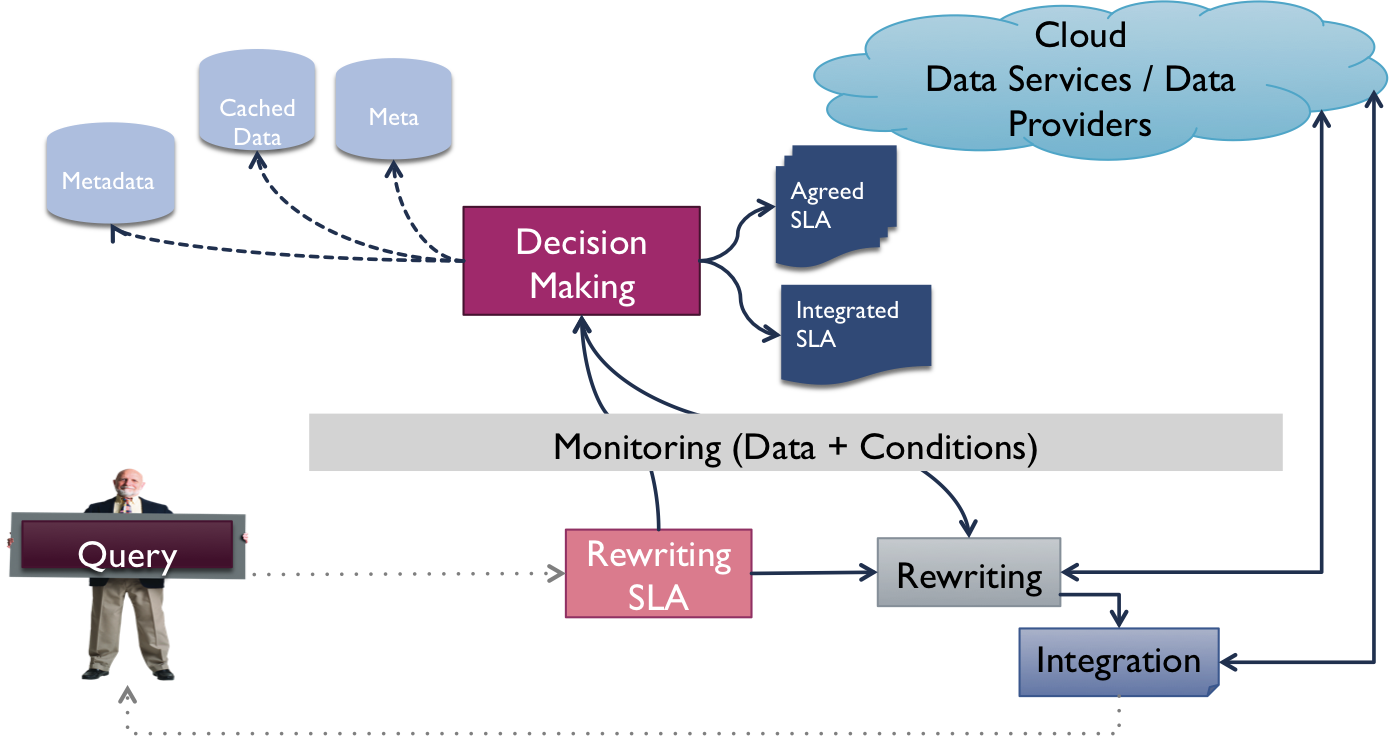
\includegraphics[width=0.5\textwidth]{figs/arch.png}
\caption{General architecture of an SLA guided  data integration system.\label{fig:arch}}
\end{figure}

Figure~\ref{fig:arch} shows the general architecture of an SLA guided data integration system that is supported by data services which are data providers deployed in a cloud and that provide agreed SLA’s. 
These descriptions are stored in a directory together with meta-data about the way queries are evaluated for producing results. 
The system uses this information  by query processing and monitoring modules for rewriting queries according to given quality of service (QoS) preferences expressed by a data consumer, for example a user.
